\chapter{The concept of black hole 2: The global view}
\label{s:glo}

\minitoc

\section{Introduction}

Having attempted in Chap.~\ref{s:def} to characterize a black hole by the local
properties of its boundary, we turn now to the general definition of a black
hole. As it could have been anticipated from the naive ``definition'' given
in Sec.~\ref{s:def:first_defin}, the mathematically meaningful definition
of a black hole cannot be local: it has to take into account the full
spacetime structure, in particular its future asymptotics. Indeed, to decide
whether a null geodesic has escaped or not, one has to wait until the ``end
of time''...

In this chapter, we therefore consider the global spacetime picture to
arrive at the general definition of a black hole in
Sec.~\ref{s:glo:def_BH}.
This amounts to focusing on the
spacetime asymptotics, which can be seen as
the region where the ``distant observers'' live and may, or may not, receive
light rays from some ``central region''. This far-away structure is best
described in terms of the so-called \emph{conformal completion}, which brings
the spacetime infinity(ies) to a finite distance in another manifold.
We start by investigating the conformal completion of the simplest
spacetime: Minkowski spacetime.

%%%%%%%%%%%%%%%%%%%%%%%%%%%%%%%%%%%%%%%%%%%%%%%%%%%%%%%%%%%%%%%%%%%%%%%%%%%%%%%%%%%%%%%%

\section{Conformal completion of Minkowski spacetime}

In this section $(\M,\w{g})$ is the 4-dimensional Minkowski spacetime,
i.e. $\M$ is a smooth manifold diffeomorphic to $\mathbb{R}^4$ and $\w{g}$
is the metric tensor whose expression in terms of some global coordinates
$(x^\alpha) = (t, x, y, z)$ implementing the diffeomorphism to $\mathbb{R}^4$
(i.e. \defin{Minkowskian coordinates}\index{Minkowskian!coordinates})
is
\be \label{e:glo:Mink_metric}
    g_{\mu\nu} \D x^\mu \D x^\nu = - \D t^2 + \D x^2 + \D y^2 + \D z^2 .
\ee

\subsection{Finite-range coordinates on Minkowski spacetime}

Since we would like to deal with the ``far'' region, it is natural to introduce
$r := \sqrt{x^2+y^2+z^2}$ and the associated spherical coordinates
$(x^\alpha) = (t,r,\th,\ph)$, which are related to the Minkowskian ones by
\be
    \left\{ \begin{array}{l}
    x = r\sin\th\cos\ph \\
    y = r\sin\th\sin\ph \\
    z = r\cos\th .
    \end{array} \right.
\ee
The coordinates $(t, r,\th,\ph)$ span
$\mathbb{R}\times(0,+\infty)\times (0,\pi) \times (0,2\pi)$; they do not cover
the whole manifold $\M$ as a regular chart (cf. Sec.~\ref{s:bas:def_manif} of Appendix~\ref{s:bas}), but only $\M\setminus \Pi$, where $\Pi$ is the closed half hyperplane defined
by $y=0$ and $x\geq 0$. Once expressed in terms of the
spherical coordinates, the Minkowski metric (\ref{e:glo:Mink_metric}) takes the form
\be
    g_{\mu\nu} \D x^\mu \D x^\nu = - \D t^2 + \D r^2
        + r^2 \left( \D\th^2 + \sin^2\th \, \D\ph^2 \right) .
\ee

\begin{figure}
\centerline{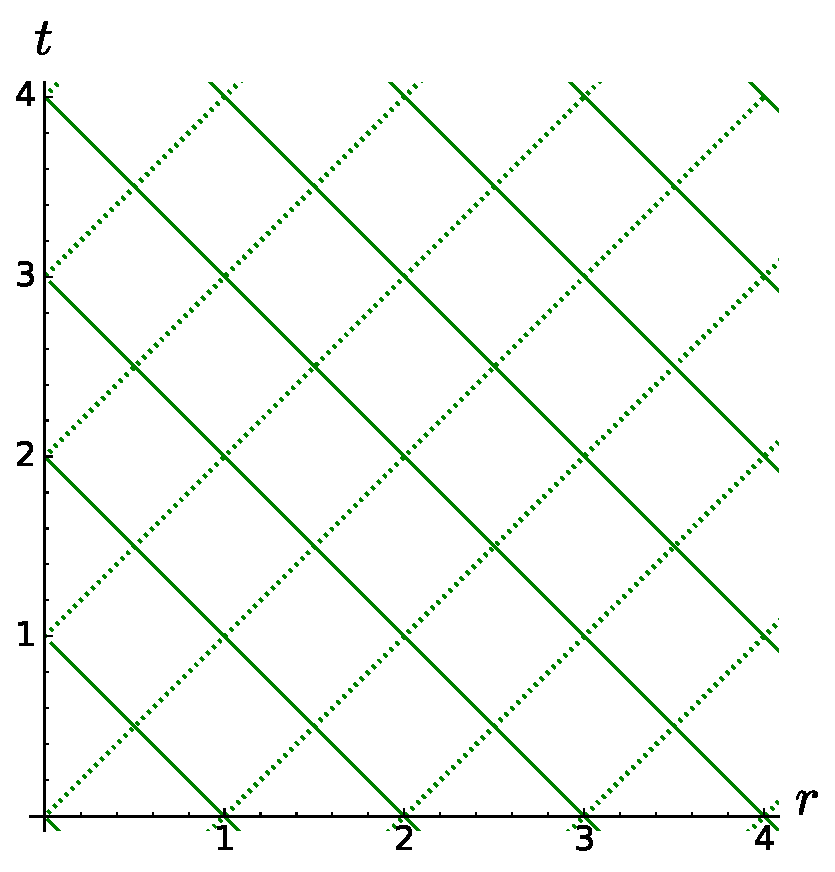
\includegraphics[width=0.5\textwidth]{glo_null_coord.pdf}}
\caption[]{\label{f:glo:glo_null_coord} \footnotesize
Lines of constant null coordinates $u$ (dashed) and $v$
(solid) in terms of the coordinates $(t,r)$.}
\end{figure}


Let us introduce the null coordinate system $(u,v,\th,\ph)$ where $u$ and
$v$ are respectively the retarted\index{retarted!time} and advanced\index{advanced!time}
time defined by (cf. Fig.~\ref{f:glo:glo_null_coord})
\be \label{e:glo:advanced_retarded}
    \left\{ \begin{array}{l}
    u = t - r\\
    v = t + r
    \end{array} \right.
    \iff
    \left\{ \begin{array}{l}
    t = \frac{1}{2} (v+u)\\[1ex]
    r = \frac{1}{2} (v-u) .
    \end{array} \right.
\ee
The metric tensor takes then the shape
\be \label{e:glo:Mink_metric_uv}
    g_{\mu\nu} \D x^\mu \D x^\nu = - \D u \, \D v
        + \frac{1}{4} (v-u)^2 \left(  \D\th^2 + \sin^2\th \, \D\ph^2 \right) .
\ee
The coordinates $(u,v)$ span the half part of $\mathbb{R}^2$ defined by
$u<v$. In order to have coordinates within a finite range, let us consider
their arctangents (cf. Fig.~\ref{f:glo:glo_atan}):
\be \label{e:glo:UV_uv}
    \left\{ \begin{array}{l}
    U = \arctan u \\
    V = \arctan v
    \end{array} \right.
    \iff
   \left\{ \begin{array}{l}
    u = \tan U \\
    v = \tan V .
    \end{array} \right.
\ee
Then the coordinates $(U,V)$ span the half part of $(-\pi/2, \pi/2)\times (-\pi/2, \pi/2)$
defined by $U < V$
(since $\arctan$ is a monotonically increasing function, cf. Fig.~\ref{f:glo:glo_atan}):
\be \label{e:glo:span_UV}
    -\frac{\pi}{2} < U < \frac{\pi}{2}, \quad
    -\frac{\pi}{2} < V < \frac{\pi}{2}, \quad\mbox{and}\quad U < V.
\ee

\begin{figure}
\centerline{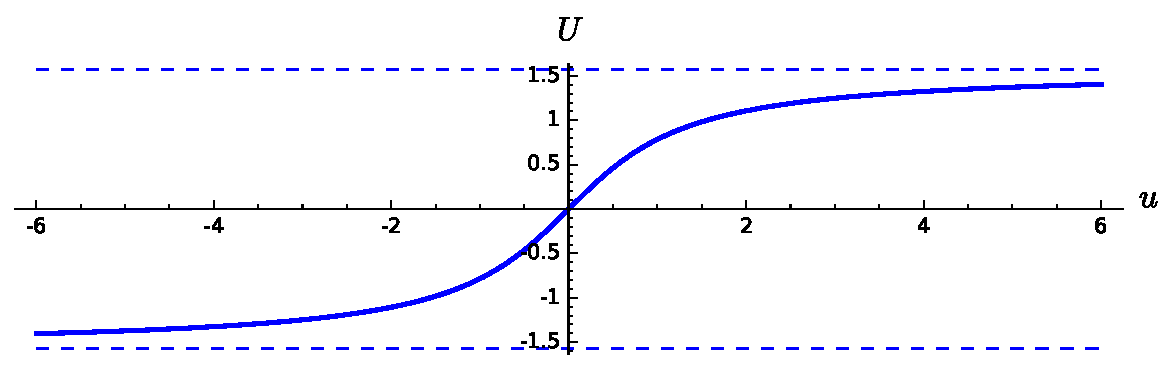
\includegraphics[width=0.8\textwidth]{glo_atan.pdf}}
\caption[]{\label{f:glo:glo_atan} \footnotesize
The arctangent function mapping $\mathbb{R}$ to $(-\pi/2, \pi/2)$.}
\end{figure}

Since
\[
    \D u = \frac{\D U}{\cos^2 U}, \quad \D v = \frac{\D V}{\cos^2 V}
    \quad\mbox{and}\quad
    \tan V - \tan U = \frac{\sin(V-U)}{\cos U \cos V},
\]
the Minkowski metric (\ref{e:glo:Mink_metric_uv})
is expressed in terms of the coordinates $(x^\alpha)=(U,V,\th,\ph)$
as\footnote{See also Sec.~\ref{s:sam:worksheets} for the computation
with SageManifolds.}
\be \label{e:glo:g_UV}
    g_{\mu\nu} \D x^\mu \D x^\nu = \frac{1}{4\cos^2 U \cos^2 V}
    \left[ - 4 \D U \, \D V + \sin^2(V-U) \left(  \D\th^2 + \sin^2\th \, \D\ph^2 \right)
    \right] .
\ee

\subsection{Conformal metric}

In the right-hand side of (\ref{e:glo:g_UV}),
the terms in square brackets defines a metric
$\w{\tilde{g}}$ such that
\be \label{e:glo:tilde_g_Omega}
    \encadre{ \w{\tilde{g}} = \Omega^2 \w{g} } ,
\ee
where $\Omega$ is the scalar field $\M \rightarrow \mathbb{R}$ obeying
\begin{subequations}
\begin{align}
    \Omega & =  2 \cos U \cos V \label{e:glo:Omega_UV} \\
           & =  \frac{2}{\sqrt{1+u^2}\sqrt{1+v^2}} \label{e:glo:Omega_uv}\\
           & =  \frac{2}{\sqrt{(t-r)^2+1}\sqrt{(t+r)^2+1}} . \label{e:glo:Omega_tr}
\end{align}
\end{subequations}
We notice on (\ref{e:glo:Omega_uv}) and (\ref{e:glo:Omega_tr}) that the function
$\Omega$ never vanishes on $\M$, so that the bilinear form $\w{\tilde{g}}$ defined by
(\ref{e:glo:tilde_g_Omega}) constitutes a well behaved metric on $\M$.
Moreover, since $\Omega^2 > 0$, $\w{\tilde{g}}$ has the same signature as
$\w{g}$, i.e. $(-,+,+,+)$.
The specific expression of $\w{\tilde{g}}$ is deduced from (\ref{e:glo:g_UV})
and (\ref{e:glo:Omega_UV}):
\be \label{e:glo:tg_UV}
    \tilde{g}_{\mu\nu} \D x^\mu \D x^\nu =  - 4 \D U \, \D V
        + \sin^2(V-U) \left(  \D\th^2 + \sin^2\th \, \D\ph^2 \right) .
\ee

In view of (\ref{e:glo:tilde_g_Omega}), one says that the metric $\w{\tilde{g}}$
is \defin{conformal to}\index{conformal} the metric $\w{g}$, or equivalently,
that the metrics $\w{g}$ and $\w{\tilde{g}}$ are
\defin{conformally related}\index{conformally related metrics},
or that $\w{\tilde{g}}$ arises from $\w{g}$ via a
\defin{conformal transformation}\index{conformal!transformation}.
The scalar field $\Omega$ is called the \defin{conformal factor}\index{conformal!factor}.

A key property of a conformal transformation is to preserve the orthogonality
relations, since (\ref{e:glo:tilde_g_Omega}) clearly
implies, at any point $p\in\M$,
\[
    \forall (\w{u},\w{v})\in T_p\M\times T_p\M,\quad
    \w{\tilde{g}}(\w{u},\w{v}) = 0 \iff \w{g}(\w{u},\w{v}) = 0 .
\]
In particular, null vectors for $\w{\tilde{g}}$ coincide with null vectors for $\w{g}$:
\[
    \forall \wl \in T_p\M,\quad
    \w{\tilde{g}}(\wl,\wl) = 0 \iff \w{g}(\wl,\wl) = 0 .
\]
Consequently the light cones of $(\M,\w{g})$ and $(\M,\w{\tilde{g}})$
are identical.
Moreover, since $\Omega^2>0$, the spacelike and timelike characters of vectors
is preserved as well:
\be
    \begin{array}{ll}
    \forall \w{v} \in T_p\M,\ &
        \w{v} \mbox{\ spacelike for\ } \w{\tilde{g}} \iff \w{v} \mbox{\ spacelike for\ } \w{g} \\
    & \w{v} \mbox{\ timelike for\ } \w{\tilde{g}} \iff \w{v} \mbox{\ timelike for\ } \w{g} .
    \end{array}
\ee
It follows that a curve $\Li$ is timelike (resp. null, spacelike) for $\w{\tilde{g}}$
iff $\Li$ is timelike (resp. null, spacelike) for $\w{g}$. Similarly,
a hypersurface $\Sigma$ is timelike (resp. null, spacelike) for $\w{\tilde{g}}$
iff $\Li$ is timelike (resp. null, spacelike) for $\w{g}$.

What about geodesics? Let us first recall that a null curve is not necessarily
a null geodesic (cf. Remark~\ref{r:def:null_curves} on page~\pageref{r:def:null_curves}),
so that one cannot deduce from the above results that conformal transformations
preserve null geodesics. However, this turns out to be true:
\begin{quote}
A smooth curve $\Li$ in $\M$ is a null geodesic for $\w{\tilde{g}}$ iff
$\Li$ is a null geodesic for $\w{g}$.
\end{quote}
To prove it, it suffices to write explicitly the geodesic equation
and to express the Christoffel symbols of $\w{\tilde{g}}$ in terms of those
of $\w{g}$ and the derivatives of $\Omega$ (see e.g. Appendix~D of Wald's
textbook \cite{Wald84} for details).

On the contrary conformal transformations preserve neither the timelike
geodesics nor the spacelike ones.

The coordinates $(U,V)$ are of null type; let us consider instead
the ``time+space'' coordinates $(\tau,\chi)$ defined by\footnote{Notice the
similarity with (\ref{e:glo:advanced_retarded}) up to some $1/2$ factors.}
\be \label{e:glo:tau_chi_U_V}
    \left\{ \begin{array}{l}
    \tau = V + U \\
    \chi = V - U
    \end{array} \right.
    \iff
    \left\{ \begin{array}{l}
    U = \frac{1}{2} (\tau - \chi) \\[1ex]
    V = \frac{1}{2} (\tau + \chi) .
    \end{array} \right.
\ee
Given (\ref{e:glo:span_UV}), the range of these new coordinates is
\be \label{e:glo:range_tau_chi}
    0 < \chi < \pi \quad\mbox{and}\quad
    \chi - \pi < \tau < \pi - \chi .
\ee
In other words, if we draw the Minkowski spacetime in the $(\tau,\chi)$ plane,
it takes the shape of a half-diamond: see Fig.~\ref{f:glo:glo_conf_diag_Mink}.

\begin{figure}
\centerline{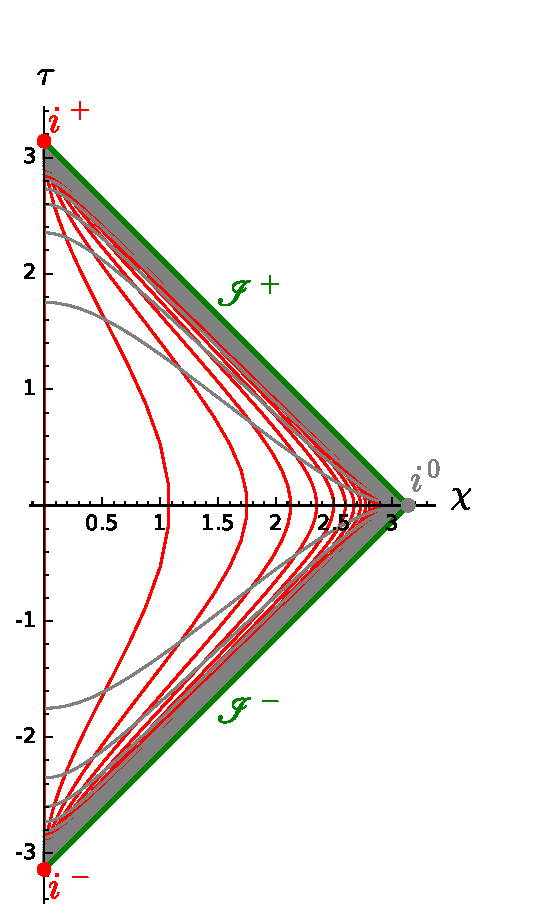
\includegraphics[width=0.5\textwidth]{glo_conf_diag_Mink.pdf}}
\caption[]{\label{f:glo:conf_diag_Mink} \footnotesize
Conformal diagram of Minkowski spacetime. Constant-$r$ curves are drawn in
red, while constant-$t$ ones are drawn in grey.}
\end{figure}

By combining (\ref{e:glo:advanced_retarded}) (\ref{e:glo:UV_uv}) and
(\ref{e:glo:tau_chi_U_V}), we get the link between $(t,r)$ and
$(\tau,\chi)$:
\be \label{e:glo:tau_chi_t_r}
    \left\{ \begin{array}{l}
    \tau = \arctan(t+r) + \arctan(t-r) \\
    \chi = \arctan(t+r) - \arctan(t-r)
    \end{array} \right.
    \iff
    \left\{ \begin{array}{l}
    \displaystyle t = \frac{\sin\tau}{\cos\tau + \cos\chi}\\[2ex]
    \displaystyle r = \frac{\sin\chi}{\cos\tau + \cos\chi} .
    \end{array} \right.
\ee
We may use these relations to draw the lines $t=\mathrm{const}$ and
$r=\mathrm{const}$ in Fig.~\ref{f:glo:glo_conf_diag_Mink}.

The expression of the conformal factor in the
coordinates $(\tau,\chi,\th,\ph)$ is easily deduced from
(\ref{e:glo:Omega_UV}) and
(\ref{e:glo:tau_chi_U_V}):
\be \label{e:glo:Omega_tau_chi}
    \Omega = \cos\tau + \cos\chi .
\ee


\subsection{Conformal completion}

The expression of the conformal metric in terms of the coordinates
$(x^\alpha) = (\tau,\chi,\th,\ph)$ is easily deduced from that in terms of
$(U,V,\th,\ph)$ as given by (\ref{e:glo:tg_UV}):
\be \label{e:glo:tg_Einstein}
    \tilde{g}_{\mu\nu} \D x^\mu \D x^\nu =  - \D\tau^2
        + \D \chi^2
        + \sin^2\chi \left(  \D\th^2 + \sin^2\th \, \D\ph^2 \right) .
\ee
Restricting to a $\tau = \mathrm{const}$ hypersurface, i.e. setting $\D\tau=0$,
we recognize the standard metric of the hypersphere
$\mathbb{S}^3$ in the hyperspherical coordinates $(\chi,\th,\ph)$.
Moreover, we notice that the full metric (\ref{e:glo:tg_Einstein})
is perfectly regular even if we relax
the condition on $\tau$ in (\ref{e:glo:range_tau_chi}), i.e. if we
let $\tau$ span the
entire $\mathbb{R}$. We may then consider the manifold
\be
    \mathscr{E} = \mathbb{R}\times \mathbb{S}^3
\ee
and $\w{\tilde{g}}$ as a Lorentzian metric on $\mathscr{E}$ given by
(\ref{e:glo:tg_Einstein}).
The Lorentzian manifold
$(\mathscr{E},\w{\tilde{g}})$ is nothing but the
\defin{Einstein static universe}\index{Einstein!static universe}\index{static!universe (Einstein)}, also called the \defin{Einstein cylinder}\index{Einstein!cylinder}\index{cylinder!Einstein --},
a static solution of the Einstein equation (\ref{e:bas:Einstein_eq})
with $\Lambda > 0$ and some pressureless matter of uniform density
$\rho = \Lambda/(4\pi)$.
We have thus a conformal isometry of Minkowski spacetime $(\M,\w{g})$ to
an open subset of the Einstein static universe $(\mathscr{E},\w{\tilde{g}})$,
that we shall denote by the same symbol $\M$.

\begin{figure}
\centerline{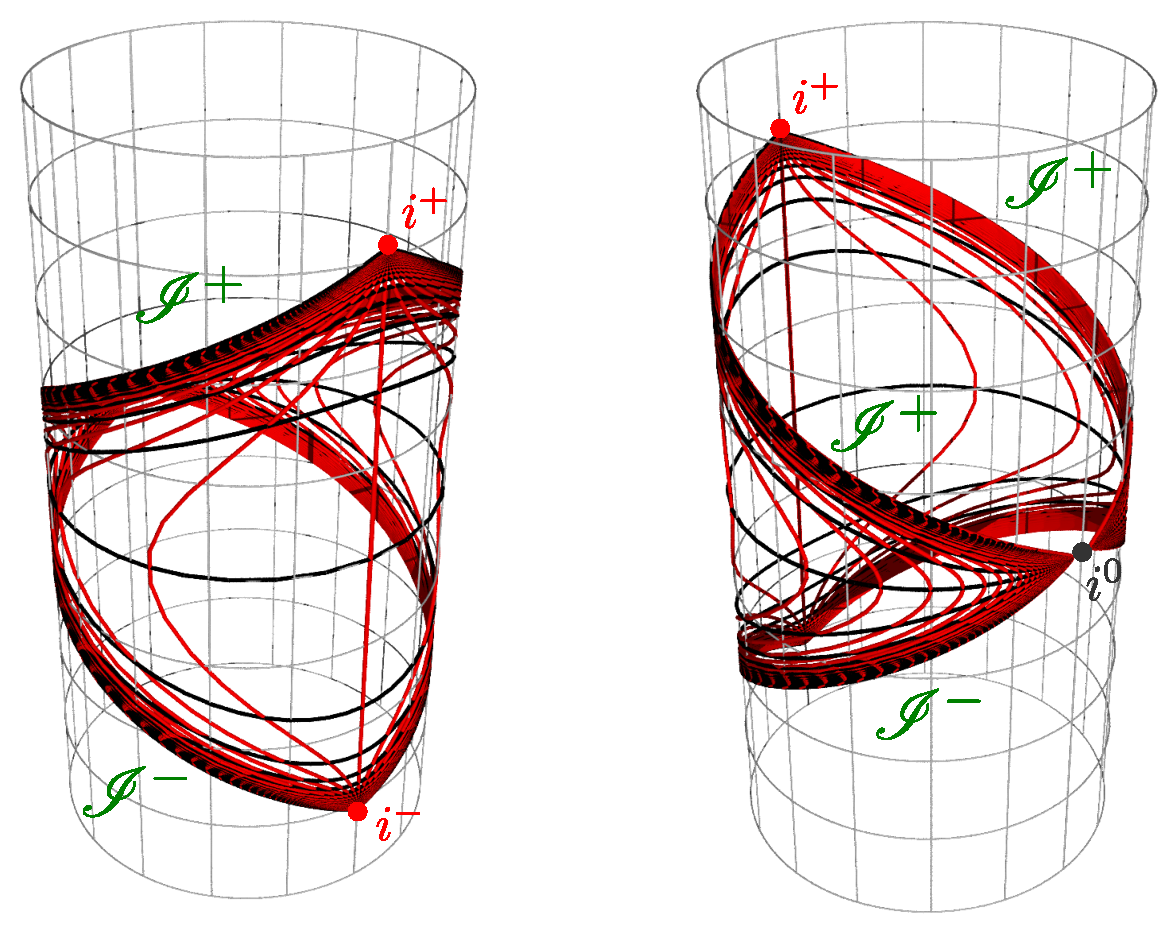
\includegraphics[width=0.6\textwidth]{glo_Einstcyl_Mink.pdf}}
\caption[]{\label{f:glo:Einstcyl_Mink}\footnotesize
Two views of the Einstein cylinder $\mathscr{E}$, with the conformal embedding of
Minkowski spacetime in it.
The red curves are the same constant-$r$ curves
as in Fig.~\ref{f:glo:conf_diag_Mink}, while the black curves are
the same constant-$t$ curves as those drawn in grey in Fig.~\ref{f:glo:conf_diag_Mink}.}
\end{figure}


The closure $\overline{\M}$ of $\M$ in $\mathscr{E}$ is (cf.
Figs.~\ref{f:glo:conf_diag_Mink} and \ref{f:glo:Einstcyl_Mink})
\be
    \overline{\M} = \M \cup \scri^+ \cup \scri^- \cup \left\{ i^0 \right\} \cup
            \left\{ i^+ \right\} \cup \left\{ i^- \right\} ,
\ee
where
\begin{itemize}
\item $\scri^+$ is the hypersurface of $\mathscr{E}$ defined by
$\tau = \pi - \chi$ and $0 < \tau < \pi$;
\item $\scri^-$ is the hypersurface of $\mathscr{E}$ defined by
$\tau = \chi - \pi $ and $-\pi  < \tau < 0$;
\item $i^0$ is the point of $\mathscr{E}$ defined by $\tau=0$ and $\chi=\pi$;
\item $i^+$ is the point of $\mathscr{E}$ defined by $\tau=\pi$ and $\chi=0$;
\item $i^-$ is the point of $\mathscr{E}$ defined by $\tau=-\pi$ and $\chi=0$.
\end{itemize}
It is customary to pronounce $\scri$ as ``scri'', for \emph{script i}.

\begin{remark}
On $\mathbb{S}^3$, the hyperspherical coordinates $(\chi,\th,\ph)$
are singular at $\chi=0$ and $\chi=\pi$, so that setting $\chi=0$ (or $\chi=\pi$)
defines a unique point of $\mathbb{S}^3$, whatever the value of $(\th,\ph)$.
Note also that the vertical left boundary of the daimond drawn in
Fig.~\ref{f:glo:glo_conf_diag_Mink}, i.e. the segment defined by
$\tau\in(-\pi,\pi)$ and $\chi=0$, is \emph{not} a part of the boundary
of $\M$ but merely reflect the coordinate singularity at $\chi=0$, in the same
way that the left vertical boundary of Fig.~\ref{f:glo:glo_null_coord}
is not a boundary of Minkowski spacetime but is
due to the coordinate singularity at $r=0$. Note by the way that
$\chi=0$ implies $r=0$ via (\ref{e:glo:tau_chi_t_r}).
\end{remark}

Let
\be
    \scri := \scri^+ \cup \scri^-
\ee
and
\be
    \tilde{\M} := \M \cup \scri .
\ee
$\tilde{\M}$ is naturally a smooth manifold with boundary\index{manifold!with boundary}
and its boundary is $\scri$:
\be
    \partial \tilde{\M} = \scri.
\ee
\begin{remark}
Because closure $\overline{\M}$ is self-intersecting at the point $i^0$
(cf. Fig.~\ref{f:glo:Einstcyl_Mink}), it is not a manifold with boundary: no open neighbourhood of
$i^0$ is homeomorphic to a neighbourhood of $[0,+\infty)\times \mathbb{R}^2$.
At the points $i^+$ and $i^-$, $\overline{\M}$ can be considered as a
topological manifold with boundary, but not as a \emph{smooth} manifold with boundary.
Hence the three points $i^0$, $i^+$ and $i^-$ are excluded from the definition
of the manifold with boundary $\tilde{\M}$.
\end{remark}

\begin{figure}
\centerline{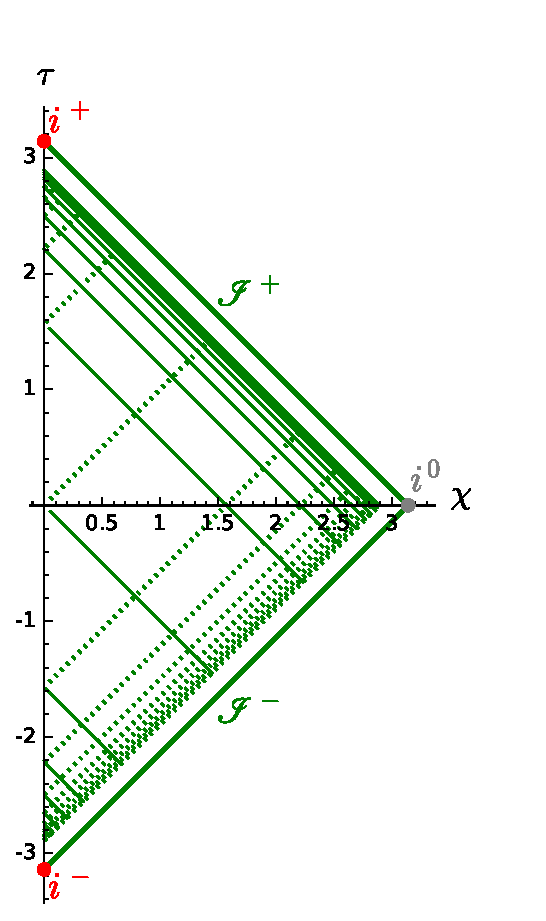
\includegraphics[width=0.45\textwidth]{glo_conf_Mink_null.pdf}}
\caption[]{\label{f:glo:conf_Mink_null}\footnotesize
Null radial geodesics in the conformal diagram of Minkowski spacetime.
The dashed green lines are null geodesics $u=\mathrm{const}$ for
17 values of $u$ uniformly spanning $[-8,8]$, while the solid green lines are
null geodesics $v=\mathrm{const}$ for 17 values of $v$ uniformly spanning $[-8,8]$.}
\end{figure}

The hypersurface $\scri^+$ is the location of $\tilde{\M}$ where all radial null geodesics
terminate, while $\scri^-$ is the location of $\tilde{\M}$ where all these geodesics orginate (cf. Fig.~\ref{f:glo:conf_Mink_null}). For this
reason $\scri^+$ is called the
\defin{future null infinity}\index{future!null infinity}\index{null!infinity}
of $(\M,\w{g})$
and $\scri^-$ the \defin{past null infinity}\index{past!null infinity}
of $(\M,\w{g})$.
On the other side, any timelike geodesic of $(\M,\w{g})$ orginates at $i\-$ and ends at
$i^+$ (cf. Fig.~\ref{f:glo:conf_diag_Mink}), while any spacelike geodesic
of $(\M,\w{g})$ originates at $i^0$ and terminates there
(after having completed a closed path on $\mathbb{S}^3$ (cf. Fig.~\ref{f:glo:Einstcyl_Mink}).
The point $i^+$ is then called the
\defin{future timelike infinity}\index{future!timelike infinity}\index{timelike!infinity}
of $(\M,\w{g})$,
$i\-$ the \defin{past timelike infinity}\index{past!timelike infinity}
of $(\M,\w{g})$
and $i^0$ the \defin{spacelike infinity}\index{spacelike!infinity} of $(\M,\w{g})$.

As it is clear on the conformal diagram of Fig.~\ref{f:glo:conf_diag_Mink},
both $\scri^+$ and $\scri^-$ are null hypersurfaces of $(\tilde{\M},\w{\tilde{g}})$.

\begin{figure}
\centerline{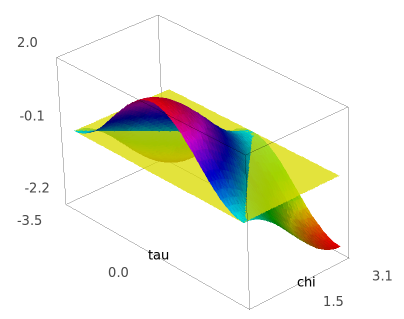
\includegraphics[width=0.45\textwidth]{glo_Omega_Mink.png}}
\caption[]{\label{f:glo:Omega_Mink}\footnotesize
Conformal factor $\Omega$ as a function of $(\tau,\chi)$ [cf. Eq.~(\ref{e:glo:Omega_tau_chi})].}
\end{figure}


It is precisely because $\Omega$ vanishes (cf. Fig.~\ref{f:glo:Omega_Mink}) at the boundary
\be
    \overline{M} - \M = \scri^+ \cup \scri^- \cup \left\{ i^0 \right\} \cup
            \left\{ i^+ \right\} \cup \left\{ i^- \right\}
\ee
that the conformal transformation (\ref{e:glo:tilde_g_Omega}) brings infinity
of Minkowski space to a finite distance.


\section{Asymptotic flatness}

A spacetime $(\M,\w{g})$ admits a
\defin{conformal completion}\index{conformal!completion}
iff there exists a Lorentzian manifold with boundary
$(\tilde{\M},\w{\tilde{g}})$ equipped with a smooth non-negative scalar field
$\Omega: \tilde{\M} \rightarrow \mathbb{R}^+$
such that
\begin{enumerate}
\item $\tilde{\M} = \M \cup \scri$, with $\scri := \partial \tilde{\M}$
(the boundary of $\tilde{\M})$;
\item on $\M$, $\w{\tilde{g}} = \Omega^2 \w{g}$;
\item on $\scri$, $\Omega=0$;
\item on $\scri$, $\dd \Omega \not= 0$;
\end{enumerate}
Condition~1 expresses that $\M$ has been endowed with some boundary,
conditions~2 and 3 express that the boundary has been brought to a
finite distance with respect to $\w{\tilde{g}}$. Finally, condition~4 ensures
that $\scri$ is a regular hypersurface of $\tilde{\M}$.

Furthermore, we shall say that $(\tilde{\M},\w{\tilde{g}})$ is a
\defin{conformal completion at null infinity}\index{conformal!completion!at null infinity}
of $(\M,\w{g})$
iff $(\tilde{\M},\w{\tilde{g}})$  is a conformal completion such that
\be
    \scri = \scri^+ \cup \scri^-,
\ee
with $\scri^+$ (resp. $\scri^-$) being never intersected by any past-directed
(resp. future-directed) causal
curve originating in $\M$.

Penrose \cite{Penro64,Penro68} has introduced the following definition:
a spacetime $(\M,\w{g})$ is \defin{asymptotically simple} iff there exists
a conformal completion $(\tilde{\M},\w{\tilde{g}})$
such that every null geodesic in $\M$ has two endpoints in $\scri$.



%%%%%%%%%%%%%%%%%%%%%%%%%%%%%%%%%%%%%%%%%%%%%%%%%%%%%%%%%%%%%%%%%%%%%%%%%%%%%%%%%%%%%%%%

\section{General definition of a black hole} \label{s:glo:def_BH}

%%%%%%%%%%%%%%%%%%%%%%%%%%%%%%%%%%%%%%%%%%%%%%%%%%%%%%%%%%%%%%%%%%%%%%%%%%%%%%%%%%%%%%%%

\section{Stationary black holes}

Hawking's strong rigity theorem
